\documentclass{thesis}

% 必要パッケージ
\usepackage{graphicx}

% メタ情報（preambleで指定）
%\setpapertitle{卒論のタイトルすごい研究 abc 123}
\setpapertitle{画像処理を用いた緊急車両の検出} 
%\setpapertitlesec{長いタイトルの場合ここに2行目を書くと2行になる}
\setadvisor{ここに姓　ここに名　教授}
\setuniv{ここに大学名　ここに学部名}
\setdept{ここに学科名}
\setyearstr{令和7年度}
\setstudentno{ここに学籍番号}
\setstudentname{ここに姓　ここに名}

\includeonly{%
chapter1,%
chapter2,%
chapter3,%
chapter4,%
chapter5,%
%Bibliography,%
shaji,
}

%−−−−−−−−−−−本文−−−−−−−−−−−− 
\begin{document}
%%%%    ここはいじらない
\makethesistitle

\frontmatter
\tableofcontents
\thispagestyle{front} 
\clearpage
\listoffigures  % 図目次を表示
\thispagestyle{front} 
\clearpage
\listoftables  % 表目次を表示
\thispagestyle{front} 
\clearpage

\mainmatter
%%%%    ここまで

%==============================================================================
%       第1章   序 論
%==============================================================================

\chapter{序  論}
\label{chapter:序論}
\typeout{1 序  論}
%%%%%%%%%%%%%%%%%%%%%%%%%%%%%%%%%%%%%%%%%%%%%%%%%%%%%%%%%%%%%%%%%%%%%%
%
%    Chapter 1  :  序論
%
\section{はじめに}
すごい研究とは何かというと，誰も思いつかない
ような役に立つことを行うことである．つまり誰で
も思いつくようなことやAI でもできるようなこと
はすごい研究ではないし，根本的にダメなのである．
すごい研究とは何かというと，誰も思いつかないよ
うな役に立つことを行うことである．つまり誰でも
思いつくようなことやAI でもできるようなことは
すごい研究ではないし，根本的にダメなのである．
すごい研究とは何かというと，誰も思いつかない
ような役に立つことを行うことである．つまり誰で
も思いつくようなことやAI でもできるようなこと
はすごい研究ではないし，根本的にダメなのである．

すごい研究とは何かというと，誰も思いつかない
ような役に立つことを行うことである．つまり誰で
も思いつくようなことやAI でもできるようなこと
はすごい研究ではないし，根本的にダメなのである．
すごい研究とは何かというと，誰も思いつかないよ
うな役に立つことを行うことである．つまり誰でも
思いつくようなことやAI でもできるようなことは
すごい研究ではないし，根本的にダメなのである．
すごい研究とは何かというと，誰も思いつかない
ような役に立つことを行うことである．つまり誰で
も思いつくようなことやAI でもできるようなこと
はすごい研究ではないし，根本的にダメなのである．

すごい研究とは何かというと，誰も思いつかない
ような役に立つことを行うことである．つまり誰で
も思いつくようなことやAI でもできるようなこと
はすごい研究ではないし，根本的にダメなのである．
すごい研究とは何かというと，誰も思いつかないよ
うな役に立つことを行うことである．つまり誰でも
思いつくようなことやAI でもできるようなことは
すごい研究ではないし，根本的にダメなのである．
すごい研究とは何かというと，誰も思いつかない
ような役に立つことを行うことである．つまり誰で
も思いつくようなことやAI でもできるようなこと
はすごい研究ではないし，根本的にダメなのである．


\section{本論文の構成}
本論文は，以下に示す5章で構成される．
第1章では，本研究の目的と概要について述べた．
第2章では，本研究の関連研究や要素技術について述べ，本研究の位置づけを明確にする．
第3章では，提案方式について述べる．
第4章では，提案方式を用いて評価し，その結果について述べ，有効性について検討する．
第5章では，本論文をまとめるとともに，今後の課題について言及する．

%%% Local Variables: 
%%% mode: latex
%%% TeX-master: t
%%% End:


%==============================================================================
%       第2章   研究の背景と本研究の位置付け
%==============================================================================

\chapter[ヘッダ用の短いタイトル]{研究の背景と本研究の位置づけなんだけど，タイトルが長すぎる場合に，ヘッダ用に短いタイトルもつけられるのです．}
\label{chapter:研究の背景と本研究の位置づけ}
\typeout{2 研究の背景と位置づけ}
%%%%%%%%%%%%%%%%%%%%%%%%%%%%%%%%%%%%%%%%%%%%%%%%%%%%%%%%%%%%%%%%%%%%%%
%
%    Chapter 2  :  研究の背景と本研究の位置付け
%
\section{携帯端末の普及}
色々普及しているよね．色々普及しているよね．色々普及しているよね．色々普及しているよね．色々普及しているよね．色々普及しているよね．色々普及しているよね．
色々普及しているよね．色々普及しているよね．色々普及しているよね．色々普及しているよね．色々普及しているよね．色々普及しているよね．色々普及しているよね．
色々普及しているよね．色々普及しているよね．色々普及しているよね．色々普及しているよね．色々普及しているよね．色々普及しているよね．色々普及しているよね．

色々普及しているよね．色々普及しているよね．色々普及しているよね．色々普及しているよね．色々普及しているよね．色々普及しているよね．色々普及しているよね．
色々普及しているよね．色々普及しているよね．色々普及しているよね．色々普及しているよね．色々普及しているよね．色々普及しているよね．色々普及しているよね．
色々普及しているよね．色々普及しているよね．色々普及しているよね．色々普及しているよね．色々普及しているよね．色々普及しているよね．色々普及しているよね．

色々普及しているよね．色々普及しているよね．色々普及しているよね．色々普及しているよね．色々普及しているよね．色々普及しているよね．色々普及しているよね．
色々普及しているよね．色々普及しているよね．色々普及しているよね．色々普及しているよね．色々普及しているよね．色々普及しているよね．色々普及しているよね．
色々普及しているよね．色々普及しているよね．色々普及しているよね．色々普及しているよね．色々普及しているよね．色々普及しているよね．色々普及しているよね．

\section{位置特定技術}

\subsection{GPS}
GPS（Global Positioning System，全地球測位システム）とは，色々あるさ．
GPS（Global Positioning System，全地球測位システム）とは，色々あるさ．
GPS（Global Positioning System，全地球測位システム）とは，色々あるさ．
GPS（Global Positioning System，全地球測位システム）とは，色々あるさ．
GPS（Global Positioning System，全地球測位システム）とは，色々あるさ．
GPS（Global Positioning System，全地球測位システム）とは，色々あるさ．
GPS（Global Positioning System，全地球測位システム）とは，色々あるさ．
GPS（Global Positioning System，全地球測位システム）とは，色々あるさ．
GPS（Global Positioning System，全地球測位システム）とは，色々あるさ．
GPS（Global Positioning System，全地球測位システム）とは，色々あるさ．
GPS（Global Positioning System，全地球測位システム）とは，色々あるさ．

\subsection{GPSGPS}
GPSGPS(GPS GPS）とは，GPSを2台使っちゃうという便利なシステムである．
GPSGPS(GPS GPS）とは，GPSを2台使っちゃうという便利なシステムである．
GPSGPS(GPS GPS）とは，GPSを2台使っちゃうという便利なシステムである．
GPSGPS(GPS GPS）とは，GPSを2台使っちゃうという便利なシステムである．
GPSGPS(GPS GPS）とは，GPSを2台使っちゃうという便利なシステムである．
GPSGPS(GPS GPS）とは，GPSを2台使っちゃうという便利なシステムである．
GPSGPS(GPS GPS）とは，GPSを2台使っちゃうという便利なシステムである．
GPSGPS(GPS GPS）とは，GPSを2台使っちゃうという便利なシステムである．
GPSGPS(GPS GPS）とは，GPSを2台使っちゃうという便利なシステムである．

\subsection{GPSGPS}
GPSGPS(GPS GPS）とは，GPSを2台使っちゃうという便利なシステムである．
GPSGPS(GPS GPS）とは，GPSを2台使っちゃうという便利なシステムである．
GPSGPS(GPS GPS）とは，GPSを2台使っちゃうという便利なシステムである．
GPSGPS(GPS GPS）とは，GPSを2台使っちゃうという便利なシステムである．
GPSGPS(GPS GPS）とは，GPSを2台使っちゃうという便利なシステムである．
GPSGPS(GPS GPS）とは，GPSを2台使っちゃうという便利なシステムである．
GPSGPS(GPS GPS）とは，GPSを2台使っちゃうという便利なシステムである．
GPSGPS(GPS GPS）とは，GPSを2台使っちゃうという便利なシステムである．
GPSGPS(GPS GPS）とは，GPSを2台使っちゃうという便利なシステムである．

\subsection{GPSGPS}
GPSGPS(GPS GPS）とは，GPSを2台使っちゃうという便利なシステムである．
GPSGPS(GPS GPS）とは，GPSを2台使っちゃうという便利なシステムである．
GPSGPS(GPS GPS）とは，GPSを2台使っちゃうという便利なシステムである．
GPSGPS(GPS GPS）とは，GPSを2台使っちゃうという便利なシステムである．
GPSGPS(GPS GPS）とは，GPSを2台使っちゃうという便利なシステムである．
GPSGPS(GPS GPS）とは，GPSを2台使っちゃうという便利なシステムである．
GPSGPS(GPS GPS）とは，GPSを2台使っちゃうという便利なシステムである．
GPSGPS(GPS GPS）とは，GPSを2台使っちゃうという便利なシステムである．
GPSGPS(GPS GPS）とは，GPSを2台使っちゃうという便利なシステムである．

\subsection{無線LAN}
無線を使ったLANである．それ以上でもそれ以下でもない．
無線を使ったLANである．それ以上でもそれ以下でもない．
無線を使ったLANである．それ以上でもそれ以下でもない．
無線を使ったLANである．それ以上でもそれ以下でもない．
無線を使ったLANである．それ以上でもそれ以下でもない．
無線を使ったLANである．それ以上でもそれ以下でもない．
無線を使ったLANである．それ以上でもそれ以下でもない．
無線を使ったLANである．それ以上でもそれ以下でもない．
無線を使ったLANである．それ以上でもそれ以下でもない．
無線を使ったLANである．それ以上でもそれ以下でもない．
無線を使ったLANである．それ以上でもそれ以下でもない．
無線を使ったLANである．それ以上でもそれ以下でもない．
無線を使ったLANである．それ以上でもそれ以下でもない．
無線を使ったLANである．それ以上でもそれ以下でもない．
無線を使ったLANである．それ以上でもそれ以下でもない．

\subsection{自律航法}
デッドレコニングですな．色々なセンサーでなんやかやとやる方式のことである，
デッドレコニングですな．色々なセンサーでなんやかやとやる方式のことである，
デッドレコニングですな．色々なセンサーでなんやかやとやる方式のことである，
デッドレコニングですな．色々なセンサーでなんやかやとやる方式のことである，
デッドレコニングですな．色々なセンサーでなんやかやとやる方式のことである，
デッドレコニングですな．色々なセンサーでなんやかやとやる方式のことである，
デッドレコニングですな．色々なセンサーでなんやかやとやる方式のことである，
デッドレコニングですな．色々なセンサーでなんやかやとやる方式のことである，
デッドレコニングですな．色々なセンサーでなんやかやとやる方式のことである，

\subsubsection{自律航法にも色々}
人生いろいろ，自律航法いろいろ．
人生いろいろ，自律航法いろいろ．
人生いろいろ，自律航法いろいろ．
人生いろいろ，自律航法いろいろ．
人生いろいろ，自律航法いろいろ．


\section{センサ類}

\subsection{加速度センサ}
加速度センサ．

\subsection{ジャイロスコープ}
ジャイロスコープ．

\subsection{地磁気センサ}
地磁気センサ．

\subsection{圧力センサ}
圧力センサ．

\subsection{近接センサ}
近接センサ．

\subsection{センサ万別}
センサ万別．

\section{機械学習}
機械学習．

\subsection{教師あり学習} 
教師あり学習．

\subsection{教師なし学習} 
教師なし学習．

\subsection{SVM}
SVM（Support vector machine）\cite{文献ABC}．


\begin{table}[t]
    \caption{表の例だよ}
    \label{tab:sample}
    \centering
    \begin{tabular}{|c||c|c|}
    \hline
     & 見出し1 & 見出し2 \\ \hline \hline
    すごい & 100 & 1000 \\ \hline
    ややすごい & 100 & 1000 \\ \hline
    とんでもない & 100 & 1000 \\ \hline
    \end{tabular}
\end{table}

\begin{figure}[t]
    \centering
    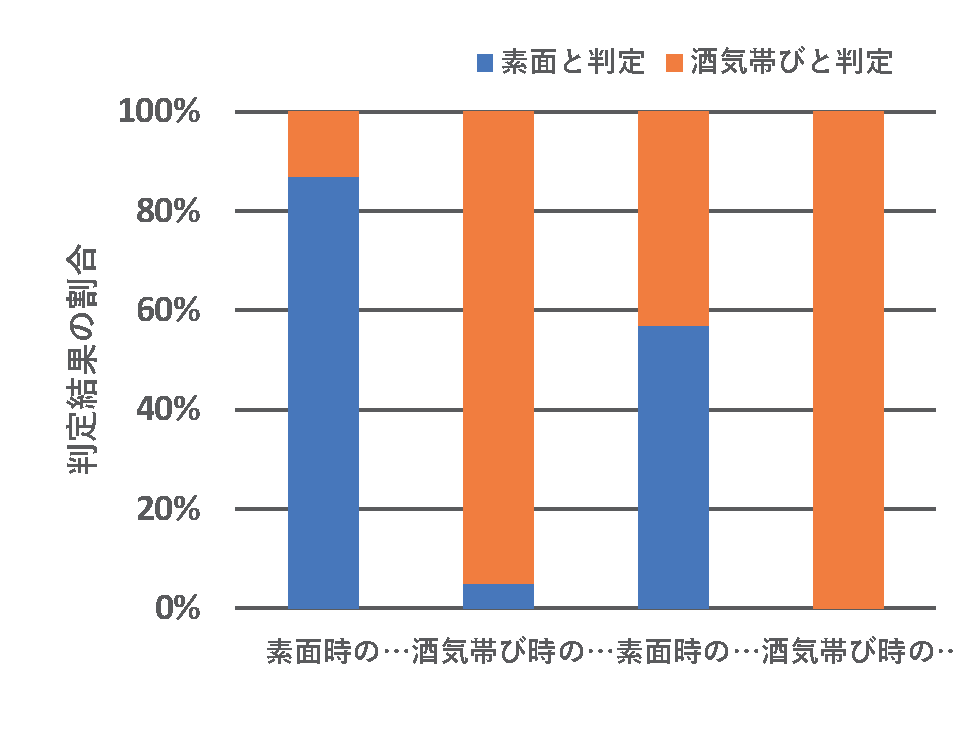
\includegraphics[width=\textwidth]{sample.eps}
    \caption{図の例．どこかにあったepsを適当に貼った}
    \label{fig:sample}
\end{figure}


\begin{table}[t]
    \caption{表の例だよ}
    \label{tab:sample2}
    \centering
    \begin{tabular}{|c||c|c|}
    \hline
     & 見出し1 & 見出し2 \\ \hline \hline
    すごい & 100 & 1000 \\ \hline
    ややすごい & 100 & 1000 \\ \hline
    とんでもない & 100 & 1000 \\ \hline
    \end{tabular}
\end{table}

\begin{figure}[t]
    \centering
    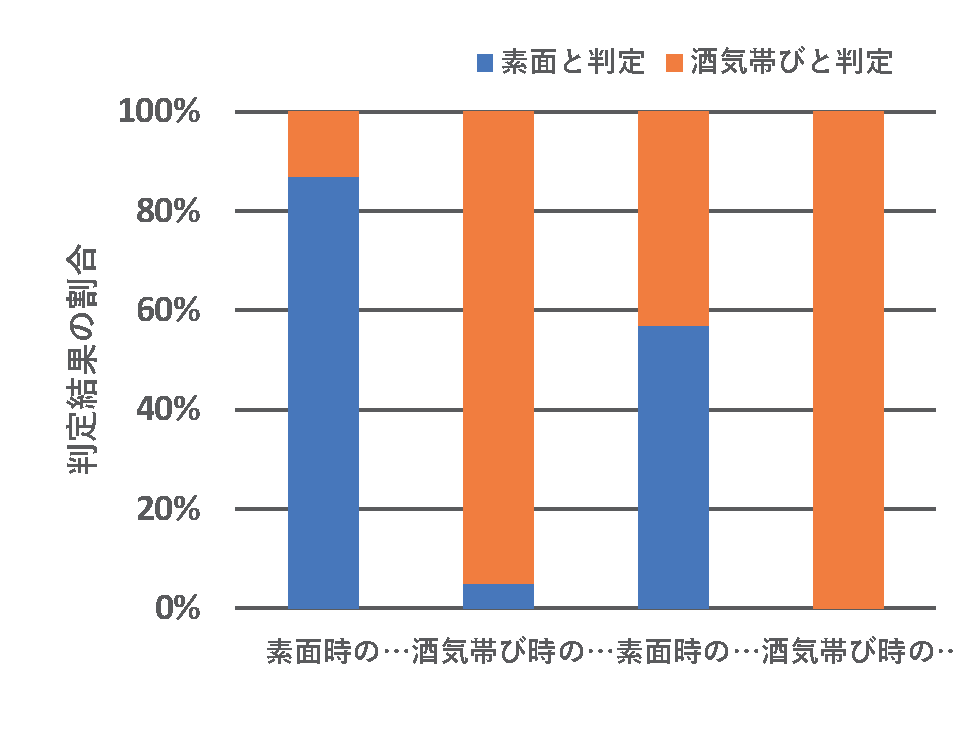
\includegraphics[width=0.7\textwidth]{sample.eps}
    \caption{図の例．どこかにあったepsを適当に貼った}
    \label{fig:sample2}
\end{figure}

\begin{table}[t]
    \caption{表の例だよ}
    \label{tab:sample3}
    \centering
    \begin{tabular}{|c||c|c|}
    \hline
     & 見出し1 & 見出し2 \\ \hline \hline
    すごい & 100 & 1000 \\ \hline
    ややすごい & 100 & 1000 \\ \hline
    とんでもない & 100 & 1000 \\ \hline
    \end{tabular}
\end{table}

\begin{figure}[t]
    \centering
    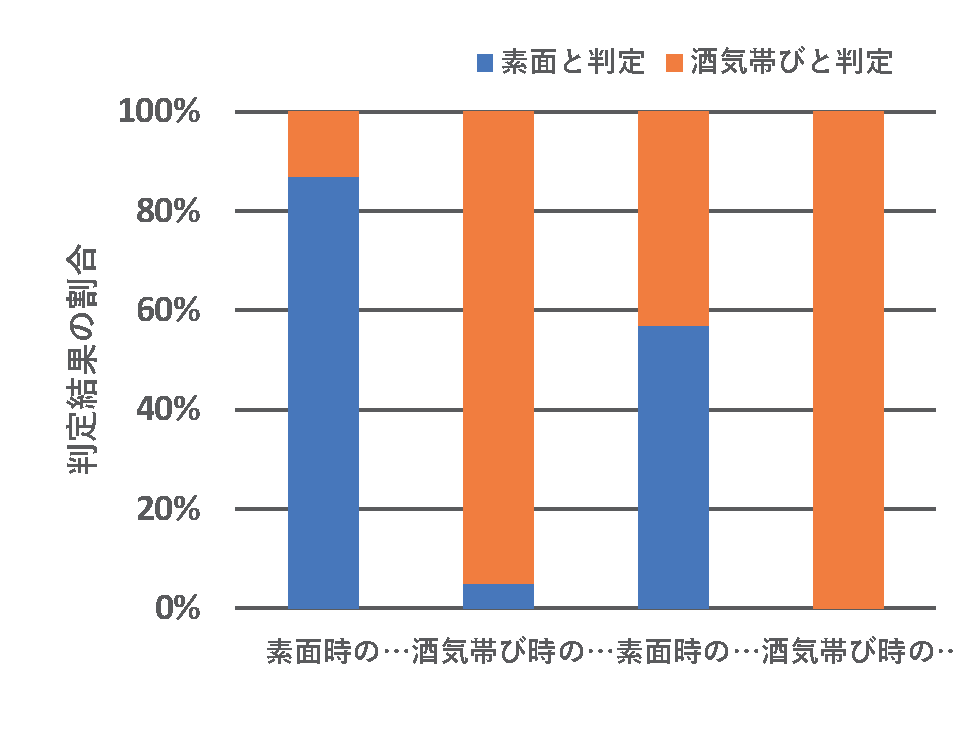
\includegraphics[width=\textwidth]{sample.eps}
    \caption{図の例．どこかにあったepsを適当に貼った}
    \label{fig:sample3}
\end{figure}



%==============================================================================
%       第3章  提案
%==============================================================================

\chapter{提案}
\label{chapter:（提案）}
\typeout{3 提案}
%%%%%%%%%%%%%%%%%%%%%%%%%%%%%%%%%%%%%%%%%%%%%%%%%%%%%%%%%%%%%%%%%%%%%%
%
%    Chapter 3  :  研究の内容
%
\section{研究内容を書きましょう}
もうサンプルを作るの疲れた．もうサンプルを作るの疲れた．
もうサンプルを作るの疲れた．もうサンプルを作るの疲れた．
もうサンプルを作るの疲れた．もうサンプルを作るの疲れた．
もうサンプルを作るの疲れた．もうサンプルを作るの疲れた．
もうサンプルを作るの疲れた．もうサンプルを作るの疲れた．
もうサンプルを作るの疲れた．もうサンプルを作るの疲れた．
もうサンプルを作るの疲れた．もうサンプルを作るの疲れた．
もうサンプルを作るの疲れた．もうサンプルを作るの疲れた．
もうサンプルを作るの疲れた．
もうサンプルを作るの疲れた．もうサンプルを作るの疲れた．
もうサンプルを作るの疲れた．もうサンプルを作るの疲れた．
もうサンプルを作るの疲れた．もうサンプルを作るの疲れた．
もうサンプルを作るの疲れた．もうサンプルを作るの疲れた．
もうサンプルを作るの疲れた．もうサンプルを作るの疲れた．
もうサンプルを作るの疲れた．もうサンプルを作るの疲れた．
もうサンプルを作るの疲れた．もうサンプルを作るの疲れた．
もうサンプルを作るの疲れた．もうサンプルを作るの疲れた．
もうサンプルを作るの疲れた．

\section{データ収集}
もうサンプルを作るの疲れた．もうサンプルを作るの疲れた．
もうサンプルを作るの疲れた．もうサンプルを作るの疲れた．
もうサンプルを作るの疲れた．もうサンプルを作るの疲れた．
もうサンプルを作るの疲れた．もうサンプルを作るの疲れた．
もうサンプルを作るの疲れた．もうサンプルを作るの疲れた．
もうサンプルを作るの疲れた．もうサンプルを作るの疲れた．
もうサンプルを作るの疲れた．もうサンプルを作るの疲れた．
もうサンプルを作るの疲れた．もうサンプルを作るの疲れた．
もうサンプルを作るの疲れた．
もうサンプルを作るの疲れた．もうサンプルを作るの疲れた．
もうサンプルを作るの疲れた．もうサンプルを作るの疲れた．
もうサンプルを作るの疲れた．もうサンプルを作るの疲れた．
もうサンプルを作るの疲れた．もうサンプルを作るの疲れた．
もうサンプルを作るの疲れた．もうサンプルを作るの疲れた．
もうサンプルを作るの疲れた．もうサンプルを作るの疲れた．
もうサンプルを作るの疲れた．もうサンプルを作るの疲れた．
もうサンプルを作るの疲れた．もうサンプルを作るの疲れた．
もうサンプルを作るの疲れた．

\begin{itemize}
\item いわゆる箇条書きってやつ
\item いわゆる箇条書きってやつ
 \begin{itemize}
    \item ネストのテスト
    \item ネストのテスト
    \item ネストのテスト
     \begin{itemize}
       \item ネストのテスト2
       \item ネストのテスト2
       \item ネストのテスト2
       \item ネストのテスト2
     \end{itemize}
    \item ネストのテスト
    \item ネストのテスト\
    \item ネストのテスト
 \end{itemize}
\item いわゆる箇条書きってやつ
     \begin{enumerate}
       \item ネストのテスト2
       \item ネストのテスト2
       \item ネストのテスト2
       \item ネストのテスト2
     \end{enumerate}
\item いわゆる箇条書きってやつ
\item いわゆる箇条書きってやつ
\item いわゆる箇条書きってやつ
\item いわゆる箇条書きってやつ
\end{itemize}

続いて\verb+enumerate+テストかな．
続いて\verb+enumerate+テストかな．
続いて\verb+enumerate+テストかな．
続いて\verb+enumerate+テストかな．
続いて\verb+enumerate+テストかな．

\begin{enumerate}
\item いわゆる箇条書きってやつ
\item いわゆる箇条書きってやつ
 \begin{enumerate}
    \item ネストのテスト
    \item ネストのテスト
    \item ネストのテスト
     \begin{enumerate}
       \item ネストのテスト2
       \item ネストのテスト2
       \item ネストのテスト2
       \item ネストのテスト2
     \end{enumerate}
    \item ネストのテスト
    \item ネストのテスト\
    \item ネストのテスト
 \end{enumerate}
\item いわゆる箇条書きってやつ
 \begin{itemize}
    \item ネストのテスト
    \item ネストのテスト
    \item ネストのテスト
     \begin{itemize}
       \item ネストのテスト2
       \item ネストのテスト2
       \item ネストのテスト2
       \item ネストのテスト2
     \end{itemize}
    \item ネストのテスト
    \item ネストのテスト\
    \item ネストのテスト
 \end{itemize}
\item いわゆる箇条書きってやつ
\item いわゆる箇条書きってやつ
\item いわゆる箇条書きってやつ
\item いわゆる箇条書きってやつ
\end{enumerate}


\subsection{使用端末}
もうサンプルを作るの疲れた．もうサンプルを作るの疲れた．
もうサンプルを作るの疲れた．もうサンプルを作るの疲れた．
もうサンプルを作るの疲れた．もうサンプルを作るの疲れた．
もうサンプルを作るの疲れた．もうサンプルを作るの疲れた．
もうサンプルを作るの疲れた．もうサンプルを作るの疲れた．
もうサンプルを作るの疲れた．もうサンプルを作るの疲れた．
もうサンプルを作るの疲れた．もうサンプルを作るの疲れた．
もうサンプルを作るの疲れた．もうサンプルを作るの疲れた．
もうサンプルを作るの疲れた．

descriptionのテスト．
\begin{description}
    \item[花の名] チューリップとか薔薇とか菜の花とか桜とか梅とか．チューリップとか薔薇とか菜の花とか桜とか梅とか．チューリップとか薔薇とか菜の花とか桜とか梅とか．チューリップとか薔薇とか菜の花とか桜とか梅とか．チューリップとか薔薇とか菜の花とか桜とか梅とか．チューリップとか薔薇とか菜の花とか桜とか梅とか．チューリップとか薔薇とか菜の花とか桜とか梅とか．チューリップとか薔薇とか菜の花とか桜とか梅とか．
    \item[都市の名] 東京とかニューヨークとか？
    \item[都市の名] 東京とかニューヨークとかロンドンとかパリとか京都とか？東京とかニューヨークとかロンドンとかパリとか京都とか？東京とかニューヨークとかロンドンとかパリとか京都とか？東京とかニューヨークとかロンドンとかパリとか京都とか？東京とかニューヨークとかロンドンとかパリとか京都とか？東京とかニューヨークとかロンドンとかパリとか京都とか？
    \item[都市の名] 東京とかニューヨークとか？
    \item[都市の名] 東京とかニューヨークとか？
    \item[都市の名] 東京とかニューヨークとか？
    \item[都市の名] 東京とかニューヨークとか？
    \item[都市の名] 東京とかニューヨークとか？
    \item[都市の名] 東京とかニューヨークとか？
    \item[都市の名] 東京とかニューヨークとか？
    \item[都市の名] 東京とかニューヨークとか？
    \item[都市の名] 東京とかニューヨークとか？
    \item[都市の名] 東京とかニューヨークとか？
\end{description}
もうサンプルを作るの疲れた．もうサンプルを作るの疲れた．
もうサンプルを作るの疲れた．もうサンプルを作るの疲れた．
もうサンプルを作るの疲れた．もうサンプルを作るの疲れた．
もうサンプルを作るの疲れた．もうサンプルを作るの疲れた．
もうサンプルを作るの疲れた．もうサンプルを作るの疲れた．
もうサンプルを作るの疲れた．もうサンプルを作るの疲れた．
もうサンプルを作るの疲れた．もうサンプルを作るの疲れた．
もうサンプルを作るの疲れた．もうサンプルを作るの疲れた．
もうサンプルを作るの疲れた．

\subsection{データ収集場所}
もうサンプルを作るの疲れた．もうサンプルを作るの疲れた．
もうサンプルを作るの疲れた．もうサンプルを作るの疲れた．
もうサンプルを作るの疲れた．もうサンプルを作るの疲れた．
もうサンプルを作るの疲れた．もうサンプルを作るの疲れた．
もうサンプルを作るの疲れた．もうサンプルを作るの疲れた．
もうサンプルを作るの疲れた．もうサンプルを作るの疲れた．
もうサンプルを作るの疲れた．もうサンプルを作るの疲れた．
もうサンプルを作るの疲れた．もうサンプルを作るの疲れた．
もうサンプルを作るの疲れた．
もうサンプルを作るの疲れた．もうサンプルを作るの疲れた．
もうサンプルを作るの疲れた．もうサンプルを作るの疲れた．
もうサンプルを作るの疲れた．もうサンプルを作るの疲れた．
もうサンプルを作るの疲れた．もうサンプルを作るの疲れた．
もうサンプルを作るの疲れた．もうサンプルを作るの疲れた．
もうサンプルを作るの疲れた．もうサンプルを作るの疲れた．
もうサンプルを作るの疲れた．もうサンプルを作るの疲れた．
もうサンプルを作るの疲れた．もうサンプルを作るの疲れた．
もうサンプルを作るの疲れた．

\begin{table}[t]
    \caption{表の例だよ}
    \label{tab:sample4}
    \centering
    \begin{tabular}{|c||c|c|}
    \hline
     & 見出し1 & 見出し2 \\ \hline \hline
    すごい & 100 & 1000 \\ \hline
    ややすごい & 100 & 1000 \\ \hline
    とんでもない & 100 & 1000 \\ \hline
    \end{tabular}
\end{table}

\begin{figure}[t]
    \centering
    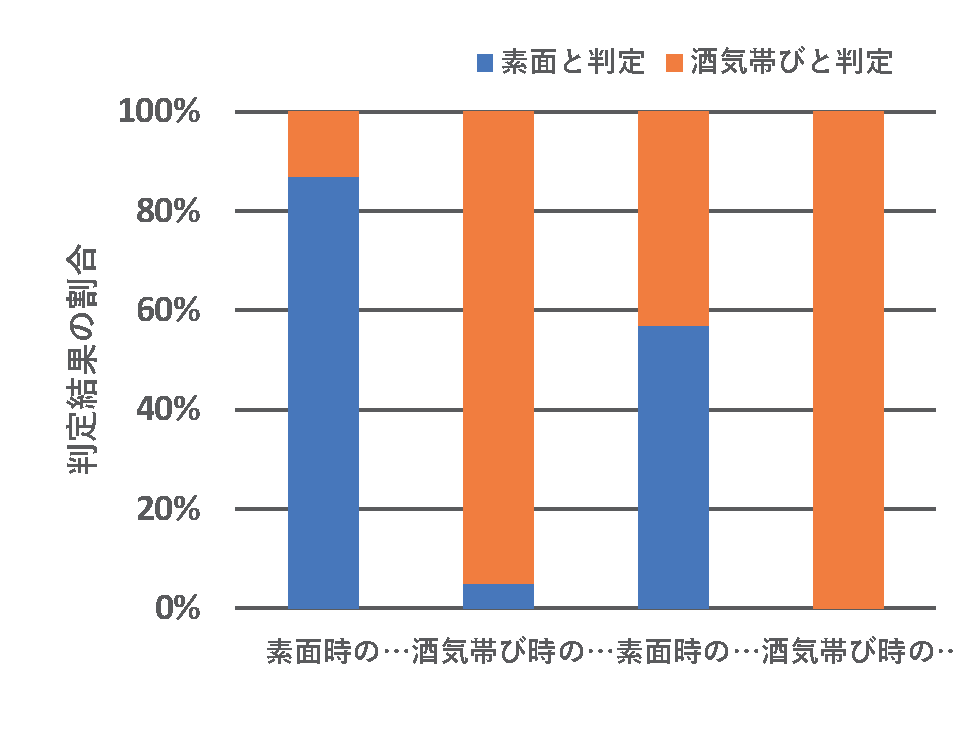
\includegraphics[width=\textwidth]{sample.eps}
    \caption{図の例．どこかにあったepsを適当に貼った}
    \label{fig:sample4}
\end{figure}


\section{提案方式}
もうサンプルを作るの疲れた．もうサンプルを作るの疲れた．
もうサンプルを作るの疲れた．もうサンプルを作るの疲れた．
もうサンプルを作るの疲れた．もうサンプルを作るの疲れた．
もうサンプルを作るの疲れた．もうサンプルを作るの疲れた．
もうサンプルを作るの疲れた．もうサンプルを作るの疲れた．
もうサンプルを作るの疲れた．もうサンプルを作るの疲れた．
もうサンプルを作るの疲れた．もうサンプルを作るの疲れた．
もうサンプルを作るの疲れた．もうサンプルを作るの疲れた．
もうサンプルを作るの疲れた．
もうサンプルを作るの疲れた．もうサンプルを作るの疲れた．
もうサンプルを作るの疲れた．もうサンプルを作るの疲れた．
もうサンプルを作るの疲れた．もうサンプルを作るの疲れた．
もうサンプルを作るの疲れた．もうサンプルを作るの疲れた．
もうサンプルを作るの疲れた．もうサンプルを作るの疲れた．
もうサンプルを作るの疲れた．もうサンプルを作るの疲れた．
もうサンプルを作るの疲れた．もうサンプルを作るの疲れた．
もうサンプルを作るの疲れた．もうサンプルを作るの疲れた．
もうサンプルを作るの疲れた．

\begin{table}[t]
    \caption{表の例だよ}
    \label{tab:sample5}
    \centering
    \begin{tabular}{|c||c|c|}
    \hline
     & 見出し1 & 見出し2 \\ \hline \hline
    すごい & 100 & 1000 \\ \hline
    ややすごい & 100 & 1000 \\ \hline
    とんでもない & 100 & 1000 \\ \hline
    \end{tabular}
\end{table}

\begin{figure}[t]
    \centering
    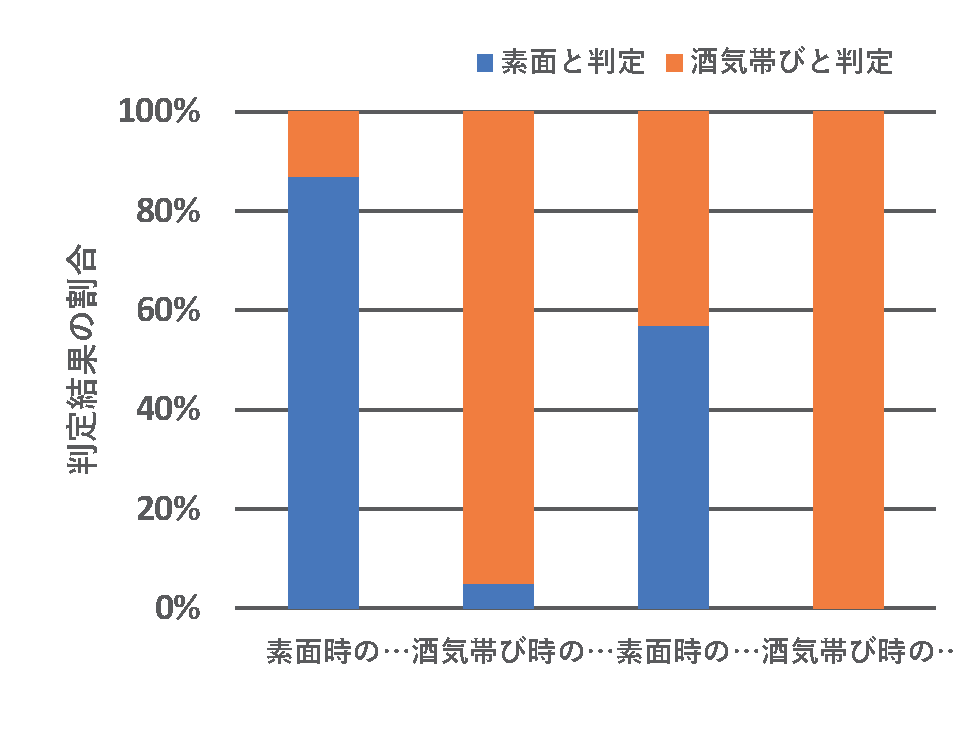
\includegraphics[width=\textwidth]{sample.eps}
    \caption{図の例．どこかにあったepsを適当に貼った}
    \label{fig:sample5}
\end{figure}



%==============================================================================
%       第4章   結果
%==============================================================================

\chapter{結果}
\label{chapter:結果}
\typeout{4 結果}
%%%%%%%%%%%%%%%%%%%%%%%%%%%%%%%%%%%%%%%%%%%%%%%%%%%%%%%%%%%%%%%%%%%%%%
%
%    Chapter 4  :  結果と評価
%

\section{結果}
もうサンプルを作るの疲れた．もうサンプルを作るの疲れた．
もうサンプルを作るの疲れた．もうサンプルを作るの疲れた．
もうサンプルを作るの疲れた．もうサンプルを作るの疲れた．
もうサンプルを作るの疲れた．もうサンプルを作るの疲れた．
もうサンプルを作るの疲れた．もうサンプルを作るの疲れた．
もうサンプルを作るの疲れた．もうサンプルを作るの疲れた．
もうサンプルを作るの疲れた．もうサンプルを作るの疲れた．
もうサンプルを作るの疲れた．もうサンプルを作るの疲れた．
もうサンプルを作るの疲れた．
もうサンプルを作るの疲れた．もうサンプルを作るの疲れた．
もうサンプルを作るの疲れた．もうサンプルを作るの疲れた．
もうサンプルを作るの疲れた．もうサンプルを作るの疲れた．
もうサンプルを作るの疲れた．もうサンプルを作るの疲れた．
もうサンプルを作るの疲れた．もうサンプルを作るの疲れた．
もうサンプルを作るの疲れた．もうサンプルを作るの疲れた．
もうサンプルを作るの疲れた．もうサンプルを作るの疲れた．
もうサンプルを作るの疲れた．もうサンプルを作るの疲れた．
もうサンプルを作るの疲れた．

\section{結果1}
もうサンプルを作るの疲れた．もうサンプルを作るの疲れた．
もうサンプルを作るの疲れた．もうサンプルを作るの疲れた．
もうサンプルを作るの疲れた．もうサンプルを作るの疲れた．
もうサンプルを作るの疲れた．もうサンプルを作るの疲れた．
もうサンプルを作るの疲れた．もうサンプルを作るの疲れた．
もうサンプルを作るの疲れた．もうサンプルを作るの疲れた．
もうサンプルを作るの疲れた．もうサンプルを作るの疲れた．
もうサンプルを作るの疲れた．もうサンプルを作るの疲れた．
もうサンプルを作るの疲れた．

\section{結果2}
もうサンプルを作るの疲れた．もうサンプルを作るの疲れた．
もうサンプルを作るの疲れた．もうサンプルを作るの疲れた．
もうサンプルを作るの疲れた．もうサンプルを作るの疲れた．
もうサンプルを作るの疲れた．もうサンプルを作るの疲れた．
もうサンプルを作るの疲れた．もうサンプルを作るの疲れた．
もうサンプルを作るの疲れた．もうサンプルを作るの疲れた．
もうサンプルを作るの疲れた．もうサンプルを作るの疲れた．
もうサンプルを作るの疲れた．もうサンプルを作るの疲れた．
もうサンプルを作るの疲れた．



%==============================================================================
%       第5章   結 論
%==============================================================================

\chapter{結  論}
\label{chapter:結論}
\typeout{5 結論}
%%%%%%%%%%%%%%%%%%%%%%%%%%%%%%%%%%%%%%%%%%%%%%%%%%%%%%%%%%%%%%%%%%%%%%
%
%    Chapter 5  :  結論
%
\label{cha:ketsuron}

もうね，ビシッと結論ですよ．
これで卒業したいわけだ．それだけの価値のある結論を示す．
もうね，ビシッと結論ですよ．
これで卒業したいわけだ．それだけの価値のある結論を示す．もうね，ビシッと結論ですよ．
これで卒業したいわけだ．それだけの価値のある結論を示す．もうね，ビシッと結論ですよ．
これで卒業したいわけだ．それだけの価値のある結論を示す．もうね，ビシッと結論ですよ．
これで卒業したいわけだ．それだけの価値のある結論を示す．もうね，ビシッと結論ですよ．
これで卒業したいわけだ．それだけの価値のある結論を示す．もうね，ビシッと結論ですよ．
これで卒業したいわけだ．それだけの価値のある結論を示す．もうね，ビシッと結論ですよ．
これで卒業したいわけだ．それだけの価値のある結論を示す．もうね，ビシッと結論ですよ．
これで卒業したいわけだ．それだけの価値のある結論を示す．もうね，ビシッと結論ですよ．
これで卒業したいわけだ．それだけの価値のある結論を示す．もうね，ビシッと結論ですよ．
これで卒業したいわけだ．それだけの価値のある結論を示す．もうね，ビシッと結論ですよ．
これで卒業したいわけだ．それだけの価値のある結論を示す．

%==============================================================================
%   謝  辞
%==============================================================================
\newpage
\section*{謝辞}
\addcontentsline{toc}{chapter}{謝辞}
\typeout{謝辞}
%\pagestyle{headings}
\markboth{謝辞}{謝辞}
\thispagestyle{front} 
%%%%%%%%%%%%%
%    謝辞
%%%%%%%%%%%%%


本研究は【ここに大学名】【ここに学部名】【ここに学科名】の【ここに研究室名】にて行われました．
本論文をまとめるにあたり，【ここに指導教員名】教授をはじめ院生の方々にご指導，ご助言，ご助力を賜わりました．
また，【ここに研究室名】の同期の方々や，【ここにキャンパス名】学生課の方々，今まで支えてくれた両親など，たくさんの方々のお陰で研究を終えることができました．
ご助力を下さった多くの方々に感謝の気持ちを表したいと思います．

\begin{flushright}
2025年 2月 \\
\end{flushright}
\newpage

\newpage

%==============================================================================
% 参考文献
%==============================================================================
\newpage
%\section*{参考文献}
\addcontentsline{toc}{chapter}{参考文献}
\typeout{参考文献}
%\pagestyle{headings}
%\markboth{参考文献}{参考文献}
\thispagestyle{front} 

\begin{thebibliography}{99}
\bibitem{yamada} 山田たろう, 「ドカベンとして生まれて」, ドカベン新書, 2023.
\bibitem{yamada2}山田たろう, 「ドカベンとして生まれて」, ドカベン新書, 2023.
\bibitem{yamada3} 山田たろう, 「ドカベンとして生まれて」, ドカベン新書, 2023.
\bibitem{yamada4} 山田たろう, 「ドカベンとして生まれて」, ドカベン新書, 2023.
\bibitem{yamada5} 山田たろう, 「ドカベンとして生まれて」, ドカベン新書, 2023.
\bibitem{yamada6} 山田たろう, 「ドカベンとして生まれて」, ドカベン新書, 2023.
\bibitem{yamada7} 山田たろう, 「ドカベンとして生まれて」, ドカベン新書, 2023.
\bibitem{yamada8} 山田たろう, 「ドカベンとして生まれて」, ドカベン新書, 2023.
\bibitem{yamada9} 山田たろう, 「ドカベンとして生まれて」, ドカベン新書, 2023.
\bibitem{yamada10} 山田たろう, 「ドカベンとして生まれて」, ドカベン新書, 2023.
\bibitem{文献ABC} 山田たろう, 「ドカベンとして生まれてABC」, ドカベン新書, 2023.
\bibitem{象の卵} 山田花子, 「象の卵はなかった」, 科研費サンプル, 2024.
\bibitem{チャッピーの大冒険} チャッピー, 「チャッピーの大冒険」, chatGPT生成, 2025.
\end{thebibliography}

\end{document}
